\documentclass{article}
\title{\huge\textbf{World Climate Change Report 2021}}
\date{\huge 2022-7-19}
\author{\huge By Nachiket Deshmukh}
\usepackage{graphicx}
\usepackage{subcaption}
\usepackage{csvsimple}
\begin{document}
\maketitle
\pagenumbering{Roman}
\newpage
\pagenumbering{arabic}

\begin{figure}
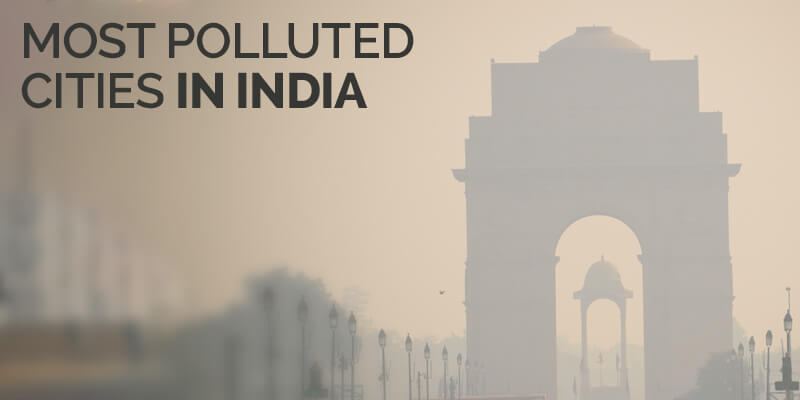
\includegraphics[width=\linewidth]{polluted_cities.jpg}
\caption{Morning Scenes in New Delhi}
\label{fig 1:Morning Scenes in New Delhi }
\end{figure}

\begin{table}[h!]
	\begin{center}
		\begin{tabular}{||c | c | c | c | c||}
		\hline
		Global Rank & Country & State & City & Avg.PM* \\
		\hline\hline
		1 & India & Rajasthan & Bhiwadi & 106.2\\ \hline
		2 & India &  Uttar Pradesh & Gaziabad & 102\\ \hline
		3 & China & Xinjiang & Hotan & 101.5\\ \hline
		4 & India & Delhi & Delhi & 96.4 \\ \hline
		5 & India & Uttar Pradesh & Jaunpur & 95.3\\ \hline
		6 & Pakistan & Punjab & Faisalabad & 94.2\\ \hline
		7 & India & Uttar Pradesh & Noida & 91.4\\ \hline
		8 & Pakistan & Punjab & Bahawalpur & 91.0\\ \hline
		9 & Pakistan & Khybar P & Peshawar & 89.6\\ \hline
		10 & India & Uttar Pradesh & Bagpat & 89.1\\ \hline
	
		
		 
		
\end{tabular}			
		
		
	\end{center}
\end{table}

\paragraph{New Delhi}The air pollution levels in India worsened in 2021, ending a three-year trend of improving air quality, according to the World Air Quality Report released by IQAir, a Swiss firm on Tuesday (March 22). India is the fifth most polluted country among 117 countries, regions and territories around the world, assessed. The country’s annual average PM2.5 levels reached 58.1 micrograms per cubic meter (µg/m3) in 2021, returning to pre-quarantine concentrations measured in 2019. The WHO recommends that average annual readings of small and hazardous airborne particles known as PM2.5 should be no more than 5 micrograms per cubic meter after changing its guidelines in 2021.

\newpage
\begin{center}
  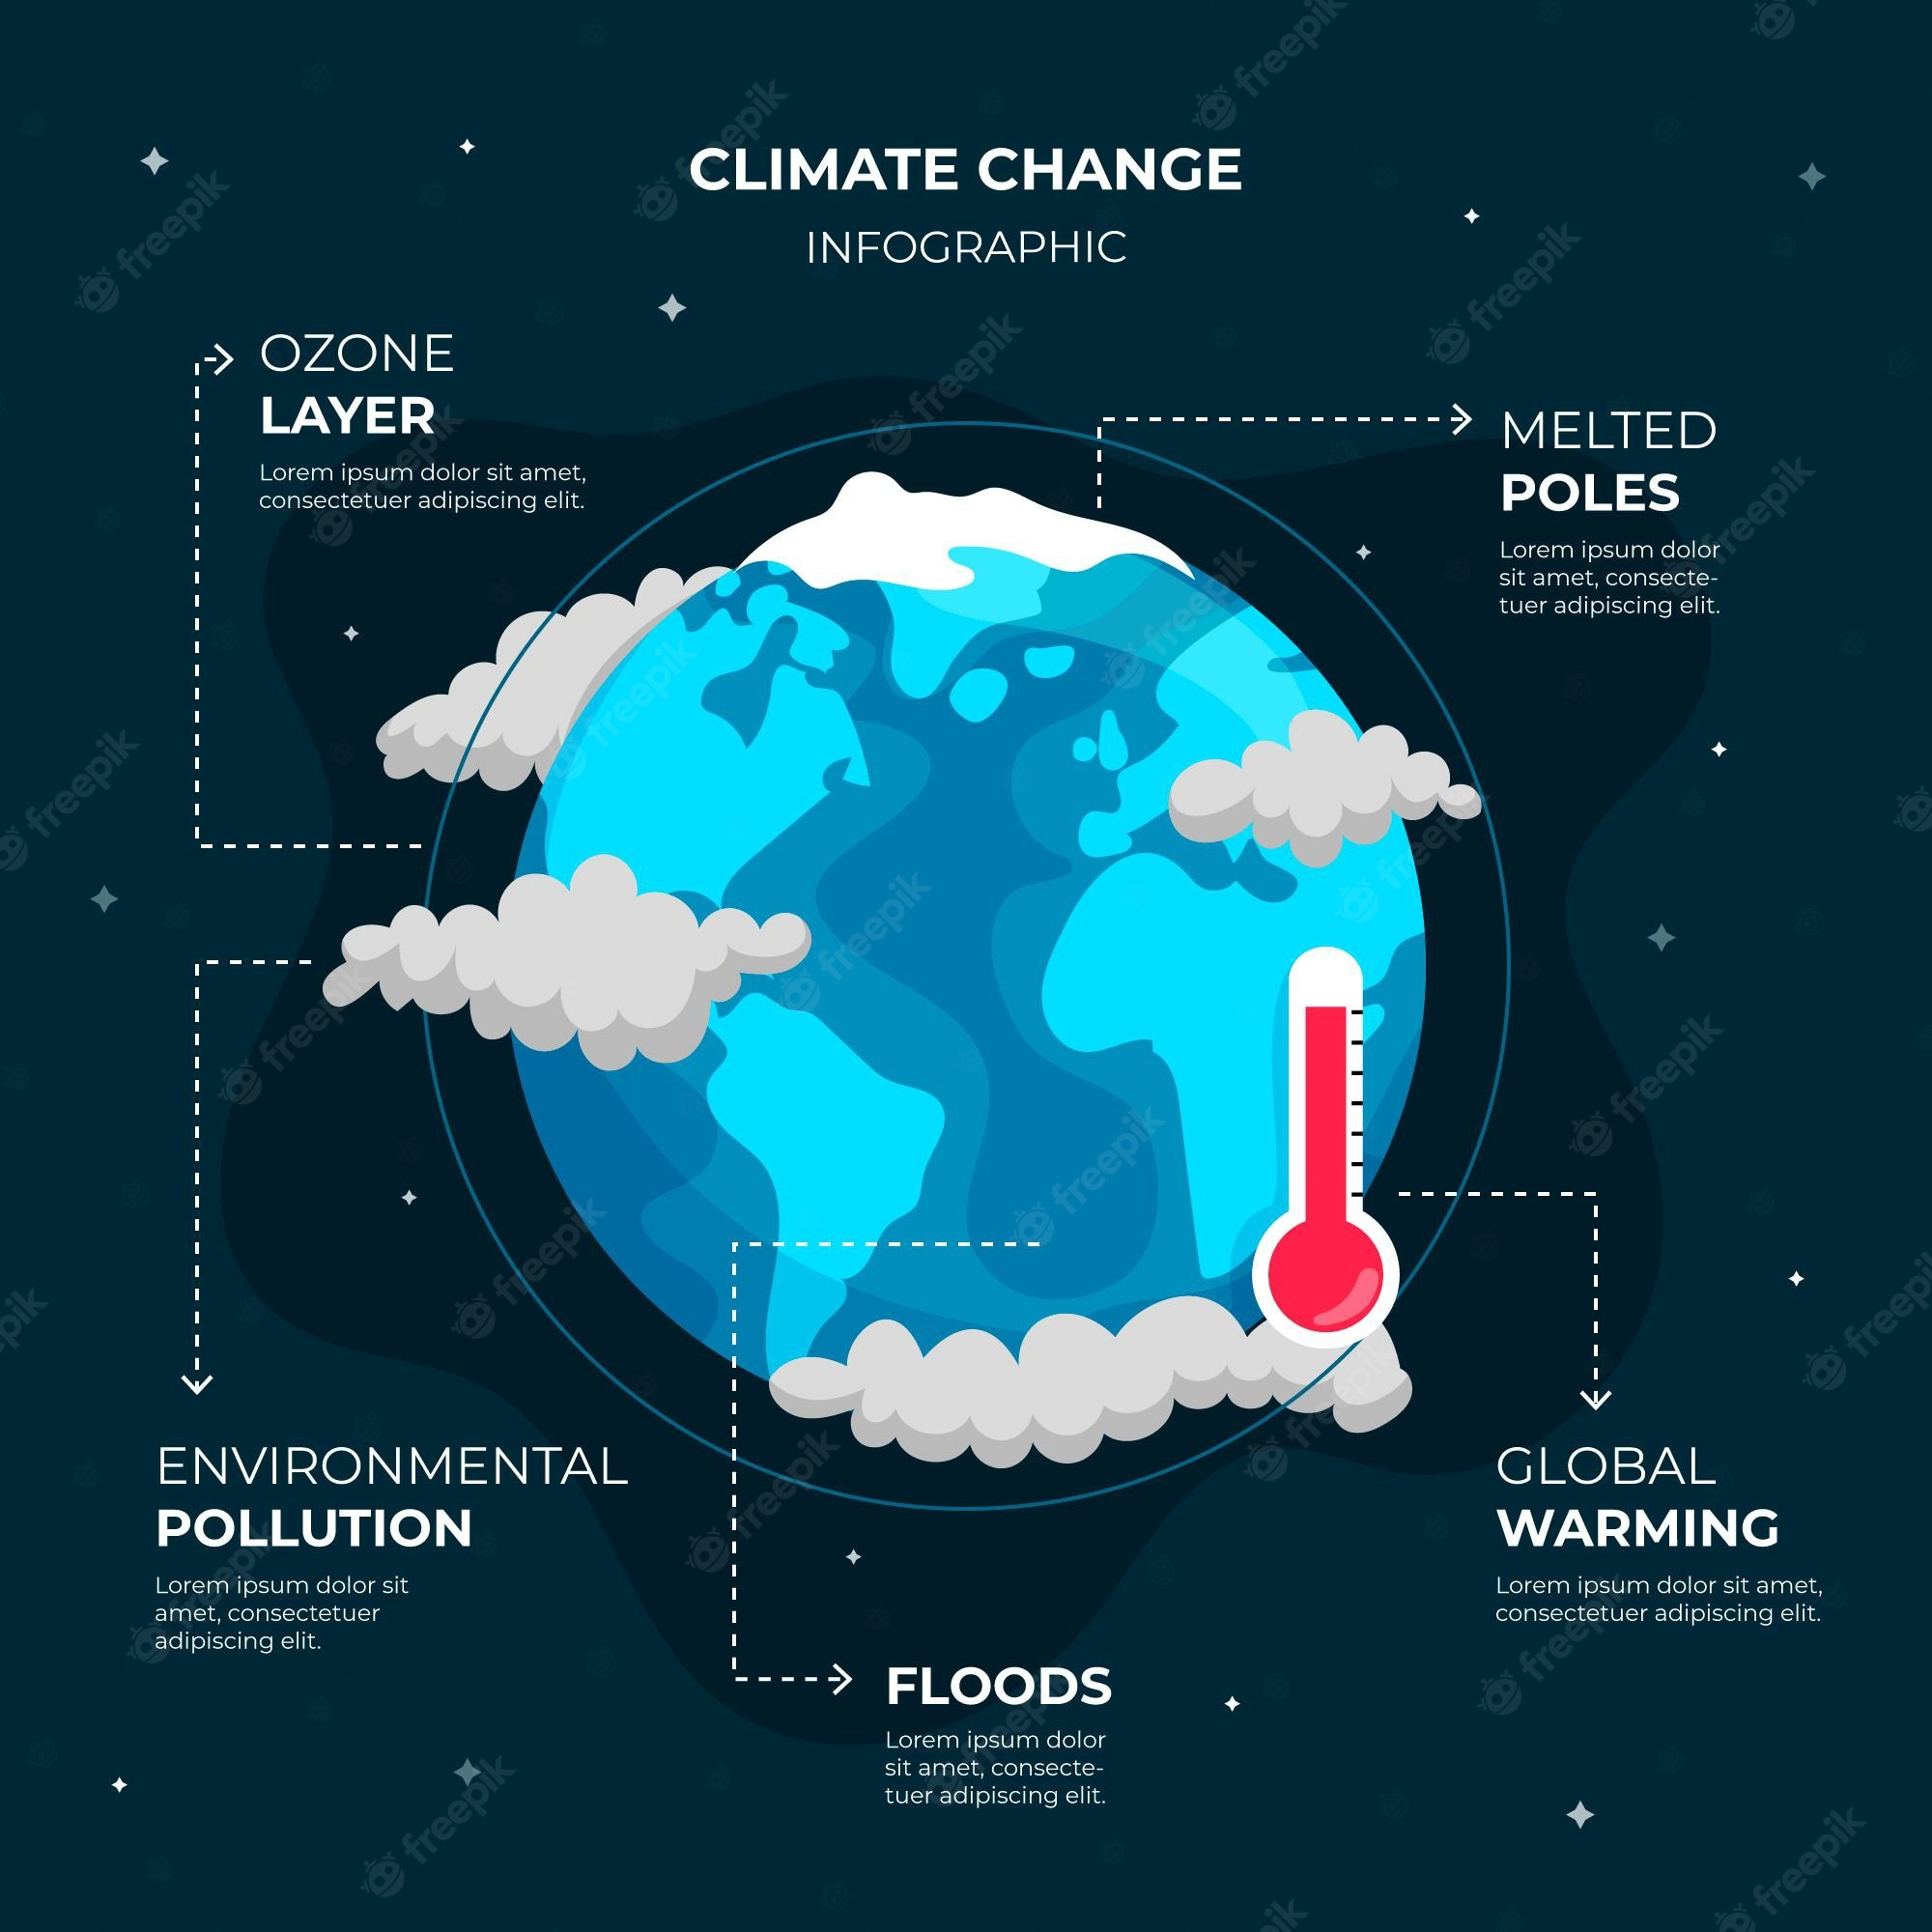
\includegraphics[width=\linewidth]{climate2.jpg}
  \label{fig:1} 
\end{center}

\begin{itemize}
\item Ozone depletion and climate change are linked in a number of ways, but ozone depletion is not a major cause of climate change.
\item Climate change, also known as global warming, is caused by a blanket of pollution that traps heat around the earth. This pollution comes from cars, factories, homes, and power plants that burn fossil fuels such as oil, coal, natural gas, and gasoline
\item Floods are made more likely by the more extreme weather patterns caused by long-term global climate change. Change in land cover—such as removal of vegetation—and climate change increase flood risk.
\end{itemize}

\newpage
Rivers and streams experience flooding as a natural result of large rain storms or spring snowmelt that quickly drains into streams and rivers.
\begin{figure}[h!]
  \centering
  \begin{subfigure}[b]{0.47\linewidth}
    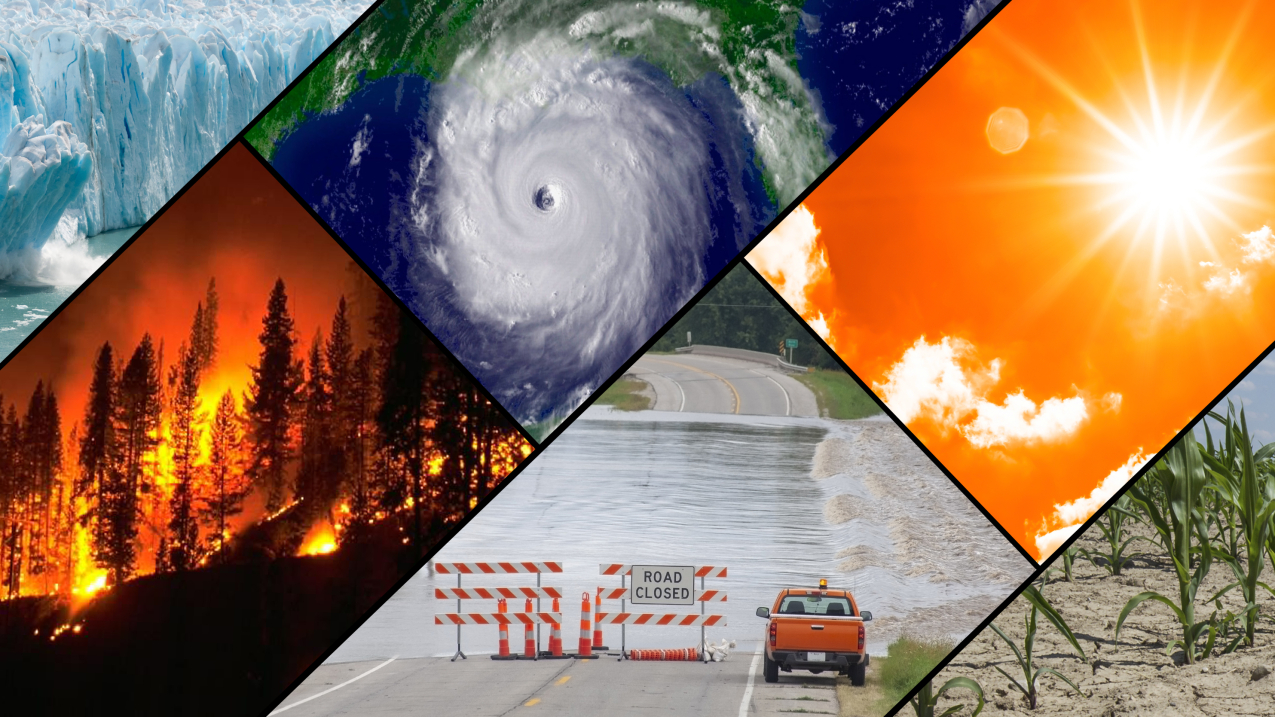
\includegraphics[width=\linewidth]{c.jpg}
    \caption{Global Warming.}
  \end{subfigure}
  \begin{subfigure}[b]{0.4\linewidth}
    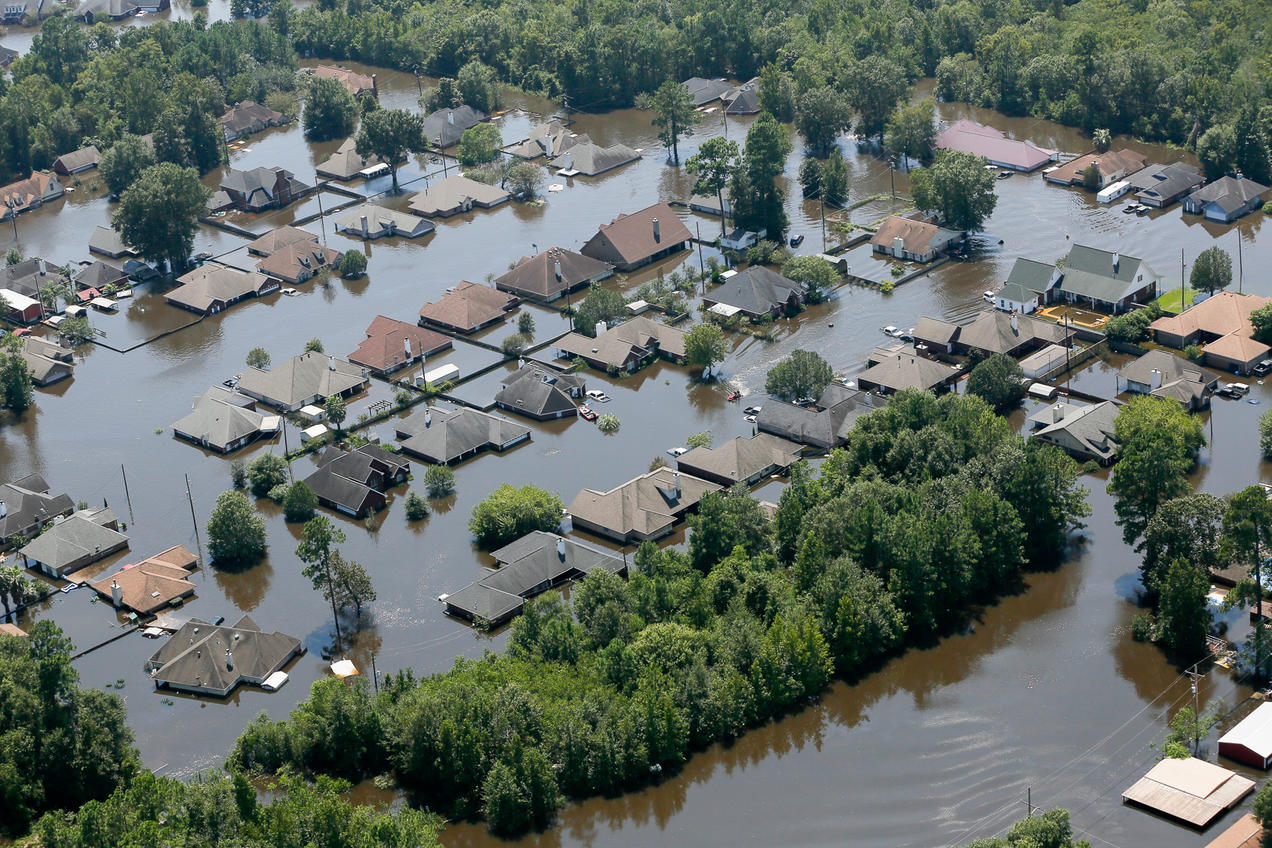
\includegraphics[width=\linewidth]{flood.jpg}
    \caption{Floods.}
  \end{subfigure}
  \caption{Shows consequences of climate change}
  \label{fig:coffee}
\end{figure}
\\
\textbf{Table using csv file}\\\\
\csvautotabular{excelfile.csv}
\end{document}